\documentclass[11pt]{article}
\usepackage[margin=0.78in]{geometry}
\usepackage{amsmath,amssymb,booktabs,graphicx,microtype,xcolor}
\usepackage[authoryear,round]{natbib}
\bibpunct{(}{)}{;}{a}{}{,}
% Match AAS's default short bibliography (article titles are kept in the .bib).
\renewcommand{\bibinfo}[2]{}
\setlength{\bibsep}{4pt}
\renewcommand{\bibfont}{\interlinepenalty=10000\urlstyle{same}}
\usepackage[hidelinks]{hyperref}
\usepackage[font=small,labelfont=bf]{caption}
\usepackage{enumitem,longtable,array}
\definecolor{atlasblue}{HTML}{176B87}
\hypersetup{colorlinks=true,linkcolor=atlasblue,citecolor=atlasblue,urlcolor=atlasblue}
\setlength{\parindent}{0pt}
\setlength{\parskip}{5pt}
\renewcommand{\topfraction}{0.95}
\renewcommand{\bottomfraction}{0.9}
\renewcommand{\textfraction}{0.05}
\renewcommand{\floatpagefraction}{0.75}
\setlist[itemize]{leftmargin=1.3em,itemsep=2pt,topsep=3pt}
\newcommand{\fedd}{f_{\mathrm{Edd}}}
\newcommand{\mbh}{M_{\mathrm{BH}}}
\newcommand{\mseed}{M_{\mathrm{seed}}}
\newcommand{\tableinput}[1]{\csname @@input\endcsname #1 }

\renewcommand{\thesection}{S\arabic{section}}
\renewcommand{\theequation}{S\arabic{equation}}
\renewcommand{\thefigure}{S\arabic{figure}}
\title{Supplementary Material: Early Black-Hole Growth Constraints from JWST}
\author{Nicole Jiang}
\date{11 September 2026}
\begin{document}
\maketitle

The main paper reports required average Eddington ratios for 224 objects in
its Balmer-line sample and 234 objects in the expanded sample. This supplement
contains the additional constant-spin grid and the early-start extrapolation.

\section{Growth equations}

We use $\fedd=L_{\rm bol}/L_{\rm Edd}$, radiative efficiency $\epsilon$,
seed mass $M_{\rm seed}$, and merger multiplier $B_{\rm merge}$.
The time available for growth is $\Delta t=t(z_{\rm obs})-t(z_{\rm seed})$.
At fixed efficiency, growth depends on the time-average $\overline{\fedd}$:
\begin{equation}
\mbh(t_{\rm obs})=B_{\rm merge}\mseed
\exp\!\left[\frac{1-\epsilon}{\epsilon}
\frac{\overline{\fedd}\,\Delta t}{t_{\rm Edd}}\right],
\label{eq:growth}
\end{equation}

\begin{equation}
\log_{10}\!\left(\frac{M_{\rm seed,req}}{M_\odot}\right)
=\log_{10}\!\left(\frac{\mbh}{M_\odot}\right)-\log_{10}B_{\rm merge}
-\frac{1-\epsilon}{\epsilon}
\frac{\overline{\fedd}\,\Delta t}{t_{\rm Edd}\ln 10}.
\label{eq:required-seed}
\end{equation}

\begin{equation}
t(z)=\frac{2}{3H_0\sqrt{\Omega_\Lambda}}
\operatorname{asinh}\!\left[\sqrt{\frac{\Omega_\Lambda}{\Omega_m}}
(1+z)^{-3/2}\right],
\label{eq:cosmictime}
\end{equation}

Here $t_{\rm Edd}=0.45$ Gyr. The age relation uses
$H_0=67.3\,{\rm km\,s^{-1}\,Mpc^{-1}}$, $\Omega_m=0.315$ and
$\Omega_\Lambda=0.685$ and neglects radiation. The main calculations begin
at $z_{\rm seed}=30$. The extension to $z=3400$ below is a mathematical
extrapolation of this age relation.

\section{Efficiency prescription}
\label{app:efficiency}

For the illustrative spin-dependent maps, the ideal Kerr thin-disk efficiency
is the ISCO binding efficiency \citep{bardeen1972}:
\begin{align}
\epsilon_a&=1-\sqrt{1-\frac{2}{3r_{\rm ISCO}}},\\
r_{\rm ISCO}&=3+Z_2-\operatorname{sgn}(a)
\sqrt{(3-Z_1)(3+Z_1+2Z_2)},\\
Z_1&=1+(1-a^2)^{1/3}\big[(1+a)^{1/3}+(1-a)^{1/3}\big],\qquad
Z_2=\sqrt{3a^2+Z_1^2}.
\label{eq:spin}
\end{align}
The dimensionless spin is $a=cJ/(G\mbh^2)$, where $J$ is the signed angular
momentum relative to the disk, and $r_{\rm ISCO}$ is in units of $G\mbh/c^2$.
The ideal efficiencies at $a=-1,0,+1$ are approximately 0.038, 0.057, and
0.423, respectively, neglecting photon capture and stress at the ISCO.
Logarithmic luminosity growth at supercritical inflow is motivated by
advection and wind models \citep{poutanen2007}. We use a simplified logarithmic relation with coefficient one and omit radial
mass loss. For Eddington ratios above unity, the maps adopt
\begin{equation}
\fedd=1+\ln\dot m,\qquad
\dot m=\frac{\dot M_{\rm in}}{L_{\rm Edd}/(\epsilon_a c^2)},\qquad
\epsilon_{\rm eff}=\begin{cases}
\epsilon_a,&\fedd\leq1,\\
\epsilon_a\fedd\exp(1-\fedd),&\fedd>1.
\end{cases}
\label{eq:effective-efficiency}
\end{equation}
The logarithmic luminosity relation applies only for super-Eddington accretion.
Each compatibility cell holds both the rate and its effective efficiency
constant over the interval. The grid tests constant accretion states with fixed spin and omits relativistic
slim-disc dynamics. For time-varying efficiency, growth depends on
$\int [(1-\epsilon(t))/\epsilon(t)]\fedd(t)\,dt$, which requires the joint
time dependence of efficiency and accretion rate.

Figure~\ref{fig:compatibility} gives the full scenario grid. The broad $10^2$--$10^6M_\odot$ interval is stored under the original code key
\nolinkurl{pbh_origin_hypothesis}. This key labels the mass interval; a primordial
interpretation requires additional assumptions about seed formation. The descriptive fractions use point masses
and the inclusive interval criterion in Section~\ref{sec:compatibility}, without error integration.
Section~\ref{app:primordial-timing} explains the conditional interpretation
of this interval for pre-existing primordial black holes.

\section{Compatibility across growth assumptions}
\label{sec:compatibility}

For each assumed accretion rate, efficiency, starting redshift and merger
contribution, we solve Eq.~\ref{eq:required-seed} for the initial seed mass
that would grow to the observed black-hole mass. We then check whether that
seed falls in each of four mass ranges: $10$--$100\,M_\odot$ (light),
$10^3$--$10^4\,M_\odot$ (intermediate), $10^4$--$10^6\,M_\odot$ (heavy),
and $10^2$--$10^6\,M_\odot$ (broad). We count an object as compatible with a
range when some seed within it can reproduce the observed mass under these assumptions. The grid uses $z_{\rm seed}=30$, three
spin/efficiency cases, merger multipliers 1 and 2, and average rates 0.3, 1
and 2. These maps use the supercritical efficiency prescription in
Section~\ref{app:efficiency}.

The seed-mass ranges overlap and are tested separately, without probability
weights. The broad range spans several possible seed-formation channels.
If the seed mass needed to reproduce an object is smaller than the lower
bound of a tested range, even the smallest seed in that range would grow
larger than the observed black hole at the assumed accretion rate. That object
is therefore excluded from the count for that range and set of growth assumptions.
For each set of assumptions, we report the percentage of catalogue objects
whose observed masses can be reproduced from a seed in the tested range.
These percentages describe this literature sample. Estimating the corresponding
percentages among all high-redshift black holes would require accounting for
how each contributing study selected and detected its objects.

The primary and exploratory samples show similar compatibility patterns
(Fig.~\ref{fig:compatibility}). For heavy seeds at $a=+1$ and $f=1$, changing
$B_{\rm merge}$ from one to two raises compatibility from 57 to 70 per cent
in the primary sample (59 to 71 per cent inclusive). At higher accretion rates, even the smallest seed in a tested mass range can
grow larger than the observed black hole. Such objects reduce the percentage
reproduced from seeds in that range.
These fractions use central mass estimates and the efficiency prescription in
Section~\ref{app:efficiency}. They describe compatibility within the selected
sample; estimating the frequency of each formation channel would require
uncertainty propagation and a population selection model.

\begin{figure}[htbp]
\centering
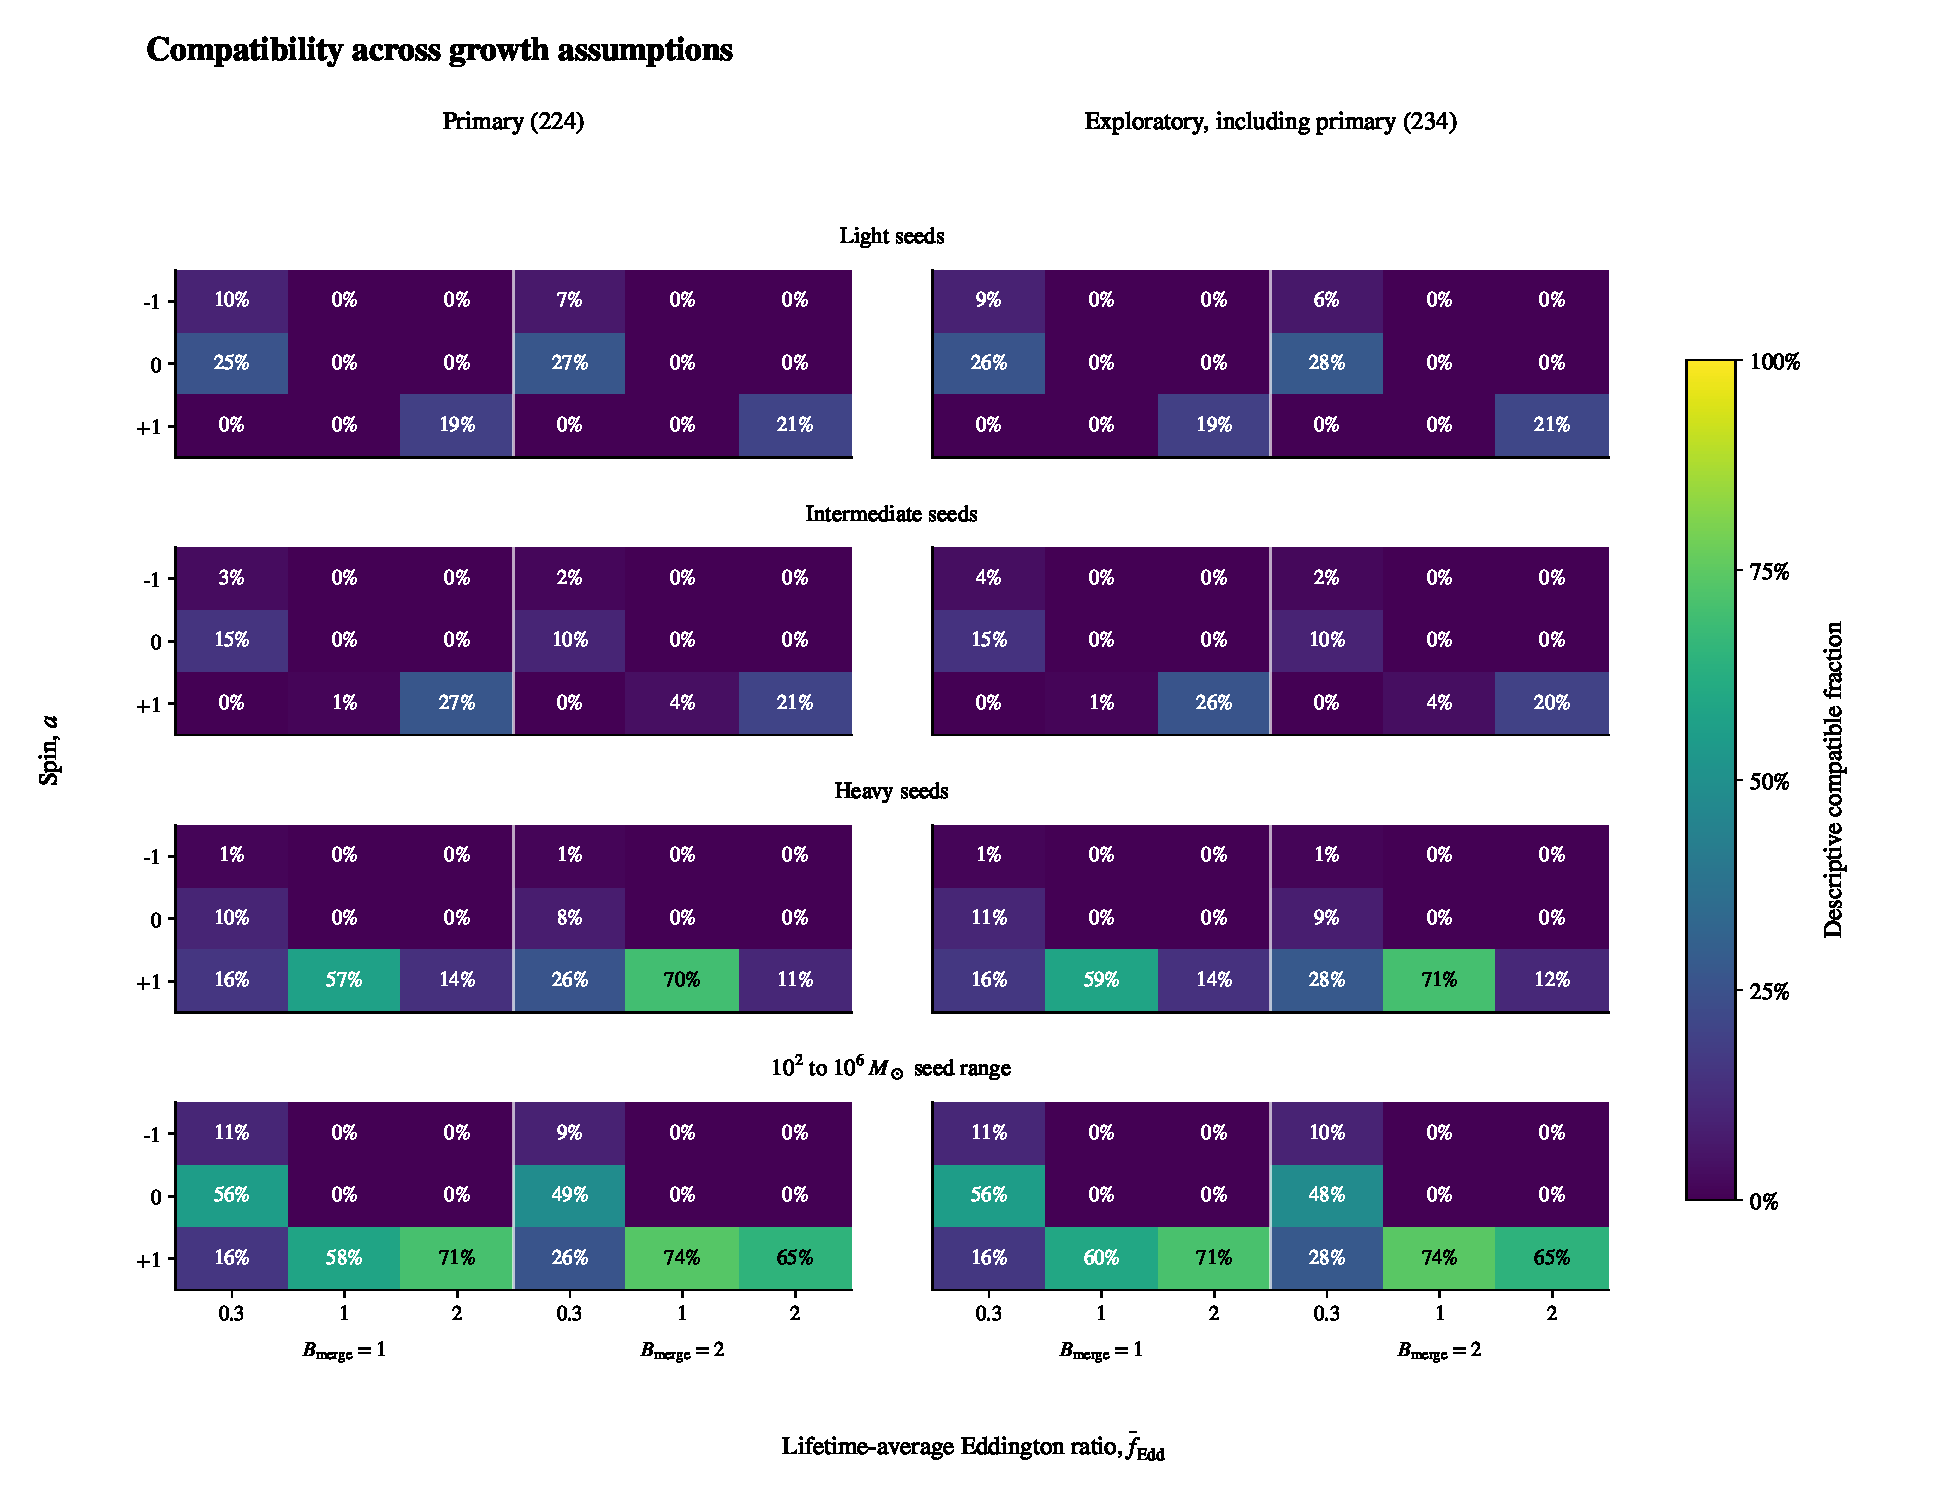
\includegraphics[width=0.99\textwidth]{figures/compatibility.pdf}
\caption{Constant-state compatibility fractions in the primary
sample (left) and the inclusive exploratory sample (right). The exploratory sample includes all primary objects. Each column specifies merger multiplier $B$ and fixed luminosity
ratio $f$; rows specify ideal spin-dependent efficiency, with the supercritical
prescription in Section~\ref{app:efficiency}. Seed intervals overlap and have no assigned probability weights. The broad
mass interval spans several possible seed-formation channels.}
\label{fig:compatibility}
\end{figure}

\section{Earlier growth onset and primordial seed interpretations}
\label{app:primordial-timing}

The growth equations take the initial mass and subsequent accretion history
as inputs. The seed-formation mechanism is left unspecified. A primordial black hole (PBH) already
present at $z=30$ can therefore be represented by its effective mass at that
epoch if it lies within the broad $10^2$--$10^6M_\odot$ interval and follows
the adopted subsequent growth prescription. This mass need not equal its
primordial formation mass. This interval covers a specified range of effective masses; inferring a
primordial origin requires a separate formation model. In \citet{dayal2024}, $z\simeq3400$ marks matter--radiation
equality and the start of the modelled evolution of PBHs that formed earlier.

Moving the start of the same constant-rate, constant-efficiency history from
$z=30$ to 3400 adds $\delta t=t(30)-t(3400)=0.09990$ Gyr in our
matter-plus-Lambda extrapolation. At fixed seed mass and merger multiplier,
the resulting shift is
\begin{equation}
\Delta\log_{10}M_{\rm BH}
=\frac{1-\epsilon}{\epsilon}
\frac{\overline{\fedd}\,\delta t}{t_{\rm Edd}\ln 10}.
\label{eq:early-start-shift}
\end{equation}
For $\overline{\fedd}=1$, this is 0.868 dex (a factor of 7.37) at
$\epsilon=0.1$, or 1.589 dex (a factor of 38.85) at the ideal non-spinning
thin-disc efficiency. The tracks shift upward by these amounts (Figure~\ref{fig:early-start}). At fixed observed mass and seed mass
requiring positive accretion, the ratio of required average rates is
$[t(z_{\rm obs})-t(30)]/[t(z_{\rm obs})-t(3400)]$; the earlier start lowers
the requirement by 6.5, 13.1 and 22.9 per cent at $z_{\rm obs}=4$, 7 and
10.603, respectively.

\begin{figure}[htbp]
\centering
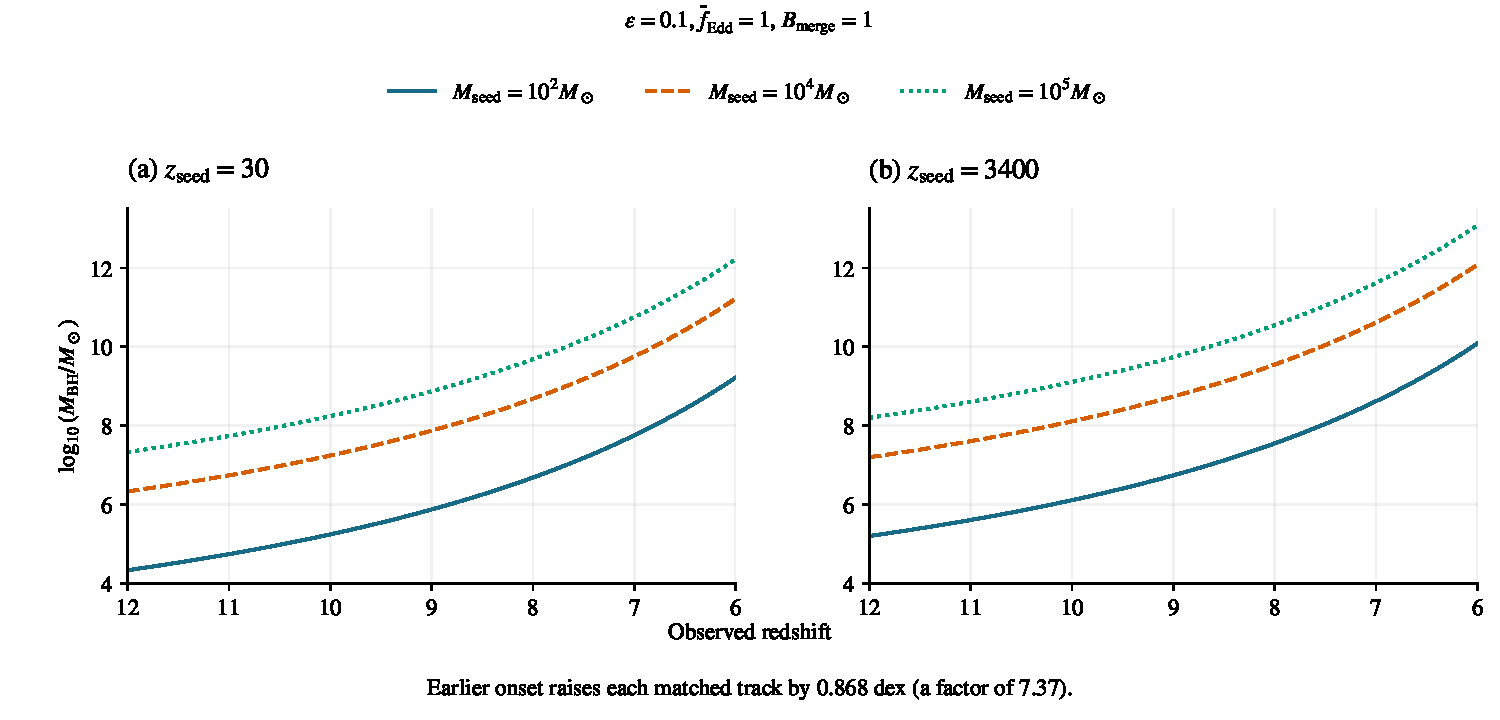
\includegraphics[width=0.99\textwidth]{figures/early_start_comparison.pdf}
\caption{Growth from $z_{\rm seed}=30$ (a) and 3400 (b), with matched
seed masses and the fixed assumptions shown. Earlier onset adds 99.90 Myr
and shifts each track upward by 0.868 dex. Here $z_{\rm seed}$ denotes the assumed start of accretion. The $z=3400$ comparison
extrapolates the matter-plus-Lambda cosmology and assumes uninterrupted
accretion. Radiation, gas supply, halo assembly and feedback are omitted.}
\label{fig:early-start}
\end{figure}

These comparisons quantify the additional growth time. Applying them to PBHs
requires an effective mass at the chosen starting epoch and a model for the
subsequent gas supply and accretion history.

\begin{thebibliography}{}
\expandafter\ifx\csname natexlab\endcsname\relax\def\natexlab#1{#1}\fi
\providecommand{\url}[1]{\href{#1}{#1}}
\providecommand{\dodoi}[1]{doi:~\href{http://doi.org/#1}{\nolinkurl{#1}}}
\providecommand{\doeprint}[1]{\href{http://ascl.net/#1}{\nolinkurl{http://ascl.net/#1}}}
\providecommand{\doarXiv}[1]{\href{https://arxiv.org/abs/#1}{\nolinkurl{https://arxiv.org/abs/#1}}}

% type= article
\bibitem[{J.~M. Bardeen {et~al.}(1972)Bardeen, Press, \&
  Teukolsky}]{bardeen1972}
Bardeen, J.~M., Press, W.~H., \& Teukolsky, S.~A. 1972,
  \bibinfo{title}{Rotating Black Holes: Locally Nonrotating Frames, Energy
  Extraction, and Scalar Synchrotron Radiation,} ApJ, 178, 347,
  \dodoi{10.1086/151796}

% type= article
\bibitem[{P. Dayal(2024)Dayal}]{dayal2024}
Dayal, P. 2024, \bibinfo{title}{Exploring a primordial solution for early black
  holes detected with JWST,} A\&A, 690, A182,
  \dodoi{10.1051/0004-6361/202451481}

% type= article
\bibitem[{J. Poutanen {et~al.}(2007)Poutanen, Lipunova, Fabrika, Butkevich, \&
  Abolmasov}]{poutanen2007}
Poutanen, J., Lipunova, G., Fabrika, S., Butkevich, A.~G., \& Abolmasov, P.
  2007, \bibinfo{title}{Supercritically accreting stellar mass black holes as
  ultraluminous X-ray sources,} MNRAS, 377, 1187,
  \dodoi{10.1111/j.1365-2966.2007.11668.x}

\end{thebibliography}
\end{document}
